\documentclass[a4paper,12pt,oneside]{article}

\usepackage[utf8]{inputenc}
\usepackage[english]{babel}
\usepackage[usenames]{xcolor}
\usepackage{etoolbox}
\usepackage{listings}
\usepackage{graphicx}
\usepackage{indentfirst}
\usepackage{makeidx}
\usepackage[unicode]{hyperref}
\usepackage{cmap}
\usepackage[T2A]{fontenc}

\hypersetup{
%bookmarks=true,            % show bookmarks bar?
%unicode=false,             % non-Latin characters in Acrobat’s bookmarks
pdfproducer={Producer},    % producer of the document
pdfkeywords={keywords},    % list of keywords
pdfnewwindow=true,         % links in new window
colorlinks=true,           % false: boxed links; true: colored links
linkcolor=black,           % color of internal links
citecolor=black,           % color of links to bibliography
    filecolor=black,           % color of file links
    urlcolor=black             % color of external links
}

\definecolor{olivegreen}{cmyk}{0.64,0,0.95,0.40}
\definecolor{mauve}{rgb}{0.58,0,0.82}

\lstset{
language=C++,                           % Code langugage
basicstyle=\ttfamily,                   % Code font, Examples: \footnotesize, \ttfamily
keywordstyle=\color{olivegreen},        % Keywords font ('*' = uppercase)
commentstyle=\color{gray},              % Comments font
stringstyle=\color{mauve},
numbers=left,                           % Line nums position
numberstyle=\tiny,
numbersep=10pt,
stepnumber=1,                           % Step between two line-numbers
frame=none,                             % A frame around the code
tabsize=2,                              % Default tab size
captionpos=b,                           % Caption-position = bottom
breaklines=true,                        % Automatic line breaking?
breakatwhitespace=false,                % Automatic breaks only at whitespace?
showspaces=false,                       % Dont make spaces visible
showstringspaces=false,
showtabs=false,                         % Dont make tabls visible
columns=flexible,                       % Column format
title=\lstname,
caption={},
extendedchars=\true,
inputencoding=utf8,
}

\begin{document}
\section{SYCL memory basics}\label{sec:Basics}

% 1. Some common words about SYCL as generic system
% 2. We will dive deeper but first we need to understand SYCL model

SYCL is a single-source programming model. This poses a problem. Normaly in heterogeneous systems, there are a diverse variety of memory types (we'll see some of them later). On the other hand, in C++ all memory is the same. So the main problem for single-source system is to find a way to somehow map one upto another.

Central ideas in this mapping are ideas of \textbf{buffer} and \textbf{accessor}. Roughly saying buffer represents GPU memory and accessor gives us a way to work with GPU memory from C++.

We will illustrate this with very basic example, which adds two vectors.

\begin{lstlisting}[caption={Vector addition with SYCL buffers},label={lst:vectoradd}]
// T const *AVec is host pointer to vector A
// the same for BVec and CVec
// size_t Sz is vector size

cl::sycl::range<1> NumOfItems{Sz};
cl::sycl::buffer<T, 1> BufferA(AVec, NumOfItems, {host_ptr});
cl::sycl::buffer<T, 1> BufferB(BVec, NumOfItems, {host_ptr});
cl::sycl::buffer<T, 1> BufferC(CVec, NumOfItems, {host_ptr});

// making calculation on GPU
DeviceQueue.submit([&](cl::sycl::handler &Cgh) {
  auto A = BufferA.template get_access<sycl_read>(Cgh);
  auto B = BufferB.template get_access<sycl_read>(Cgh);
  auto C = BufferC.template get_access<sycl_write>(Cgh);

  auto Kern = [A, B, C](cl::sycl::id<1> wiID) {
    C[wiID] = A[wiID] + B[wiID];
  };
  Cgh.parallel_for<class vector_add_buf<T>>(NumOfItems, Kern);
});

// checking with host calculations
auto A = BufferA.template get_access<sycl_read>();
auto B = BufferB.template get_access<sycl_read>();
auto C = BufferC.template get_access<sycl_read>();

for (int I = 0; I < Sz; ++I)
  if (C[I] != A[I] + B[I]) {
    std::cerr << "At index: " << I << ". ";
    std::cerr << C[I] << " != " << A[I] + B[I] << "\n";
    std::terminate();
  }
\end{lstlisting}

Here things are somewhat abbreviated (SYCL often requires really long namespace chains).

\begin{lstlisting}
// buffer attribute
constexpr auto host_ptr = 
    cl::sycl::property::buffer::use_host_ptr{};

// accessor types
constexpr auto sycl_read = cl::sycl::access::mode::read;
constexpr auto sycl_write = cl::sycl::access::mode::write;
\end{lstlisting}

This is buffer attribute, showing, that buffer have underlying host pointer. Also we have accessor type abbreviations for read-only and write-only things.

Next we create buffer, which is sort of handle to GPU memory. On creation we explicitly tell which part of CPU memory to take and send to GPU.

\begin{lstlisting}
cl::sycl::range<1> NumOfItems{Sz};
cl::sycl::buffer<T, 1> bufferA(AVec, NumOfItems, {host_ptr});
\end{lstlisting}

We are specifying host pointer, range, and leaving everything else to SYCL API. Now our buffer have its representative in the SYCL world. It will manage data and send it back and forth if required. If we do not want it to write back after kernel is done, we can block writeback explicitly.

\begin{lstlisting}
BufferA.set_final_data(nullptr);
\end{lstlisting}

Now we are getting an \textbf{accessor} A. Accessors are C++ objects, acting as pointers to the corresponding address space. There is no notion of address space in C++, so we need this abstract layer to fill the gap.

\begin{lstlisting}
auto Evt = DeviceQueue.submit([&](cl::sycl::handler &Cgh) {
// .....
  auto A = BufferA.template get_access<sycl_read>(Cgh);
\end{lstlisting}

Which kind of memory are pointed-to by this accessor? Inside \lstinline!cl::sycl::buffer!, method \lstinline!get_access! returns accessor to global memory only. That is why now we will limit ourselves only with different flavors of global memory. For other memory kinds, see (\ref{subsec:PrivLocal}) and later. Inside offload working with such accessor, indexed by SYCL id is much like working with host pointer, indexed by integral value.

\begin{lstlisting}
auto Kern = [A, B, C](cl::sycl::id<1> wiID) {
  C[wiID] = A[wiID] + B[wiID];
};
Cgh.parallel_for<class vector_add_buf<T>>(NumOfItems, Kern);
\end{lstlisting}

At first glance this looks slightly overcomplicated? Yes, it should. For some reasons we need:

\begin{itemize}
\item Create buffer from host pointer. Capture this buffer to device queue submit.
\item Get accessor from buffer. Capture this accessor to kernel lambda. At this point you have some idea about which type of memory you are addressing.
\item Use accessor inside kernel lambda, index it by workitem id.
\end{itemize}

Even more: we can have this line, getting an accessor not only inside device queue. We might have it in host code, after we have writeback to buffer \lstinline!C!.

\begin{lstlisting}
auto C = BufferC.template get_access<sycl_read>();
\end{lstlisting}

Host-side accessor also behaves like pointer with same indexing operator and we can check on host side that everything is correct.

Is it the only way? Can we do things different? Lets start investigating...

\subsection{Host, device and shared memory}\label{subsec:HostDevice}

% 1. Explicit and implicit memory send back and forth
% 2. Shared memory may be really efficient for integrated GPUs

\begin{figure}
\centering
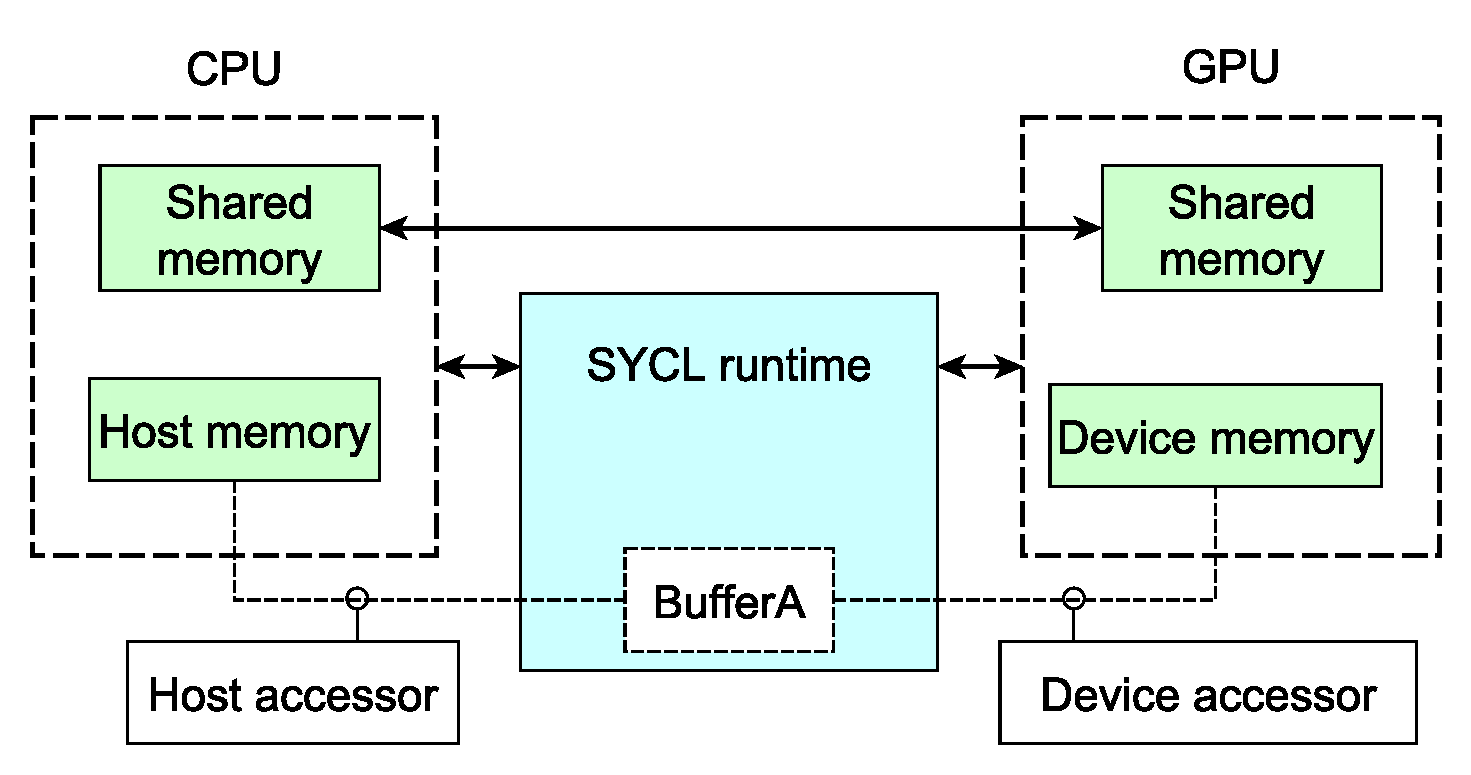
\includegraphics[width=1.0\textwidth]{pictures/sycl-device-and-shared-mem.pdf}
\caption{SYCL device and shared memory}
\label{fig:sycl-device-and-shared-mem}
\end{figure}

Figure (\ref{fig:sycl-device-and-shared-mem}) represents our first, rather naive mental model of host, device and shared memory. You may think that GPU have its own memory onboard, and CPU does as well. So when you are working with buffers as we did in example to (\ref{sec:Basics}), you explicitly instruct SYCL runtime when to move memory from CPU to GPU and when to read results back.

SYCL runtime also builds implicit task graph, based on accessors and schedules tasks, honoring access dependencies. This is not really about memory, so lets pass this topic for now.

Other way to write vector add is to write it using \textbf{shared memory}.

\begin{lstlisting}[caption={Vector addition in shared memory},label={lst:vectoraddshared}]
auto *A = cl::sycl::malloc_shared<T>(Sz, DeviceQueue);
auto *B = cl::sycl::malloc_shared<T>(Sz, DeviceQueue);
auto *C = cl::sycl::malloc_shared<T>(Sz, DeviceQueue);

// copy to shared memory
std::copy(AVec, AVec + Sz, A);
std::copy(BVec, BVec + Sz, B);

DeviceQueue.parallel_for(numOfItems,
    [=](auto n) { C[n] = A[n] + B[n]; });

DeviceQueue.wait();

// copy back to normal memory
std::copy(C, C + Sz, CVec);
\end{lstlisting}

In this case you are not telling device queue to create buffers or accessors. Instead you just order to put everything in shared memory and let hardware to synchronize this memory in the background.

% TODO: gnuplot data from bitonic sort example? Need to think about it...

\subsection{Private, local and global memory}\label{subsec:PrivLocal}

% 1. SYCL accessors: global and local
% 2. Glorious GEMM example 
% 3. Private memory for explicit workgroup

Any modern GPU (at least those, produced by NVidia, AMD and Intel) have notion of shared local memory and private memory. In abstract model of SYCL this is simple: we have work-items and each work-item have small amount of private memory. Work-items are combined in work-groups, each item within work-group have shared access to bigger amount of local memory and finally all work-items have shared access to global memory as represented on (fig. \ref{fig:sycl-privatemem}).

\begin{figure}
\centering
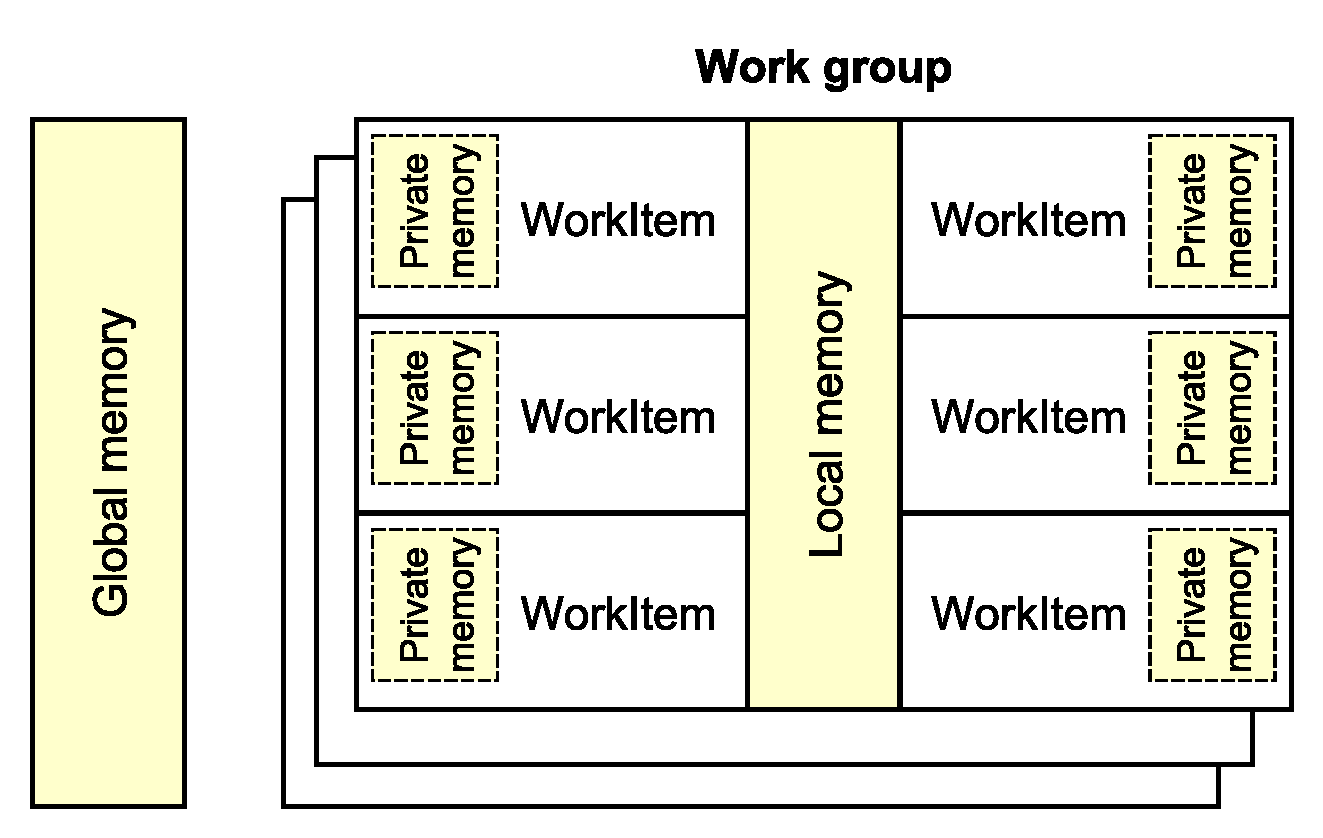
\includegraphics[width=1.0\textwidth]{pictures/sycl-privatemem.pdf}
\caption{SYCL global, local and private memory}
\label{fig:sycl-privatemem}
\end{figure}

In this sense, shared virtual memory is also (logically) a kind of global memory, since it is accessible to all work-items.

Basic example on how private memory affects performance is GEMM example.

In matrix multiplication iteration space is a cell of the resulting matrix, so each workitem as shown on (fig. \ref{fig:iter-space-matrix}) basically does dot product of vectors and then accumulate results. 

\begin{figure}
\centering
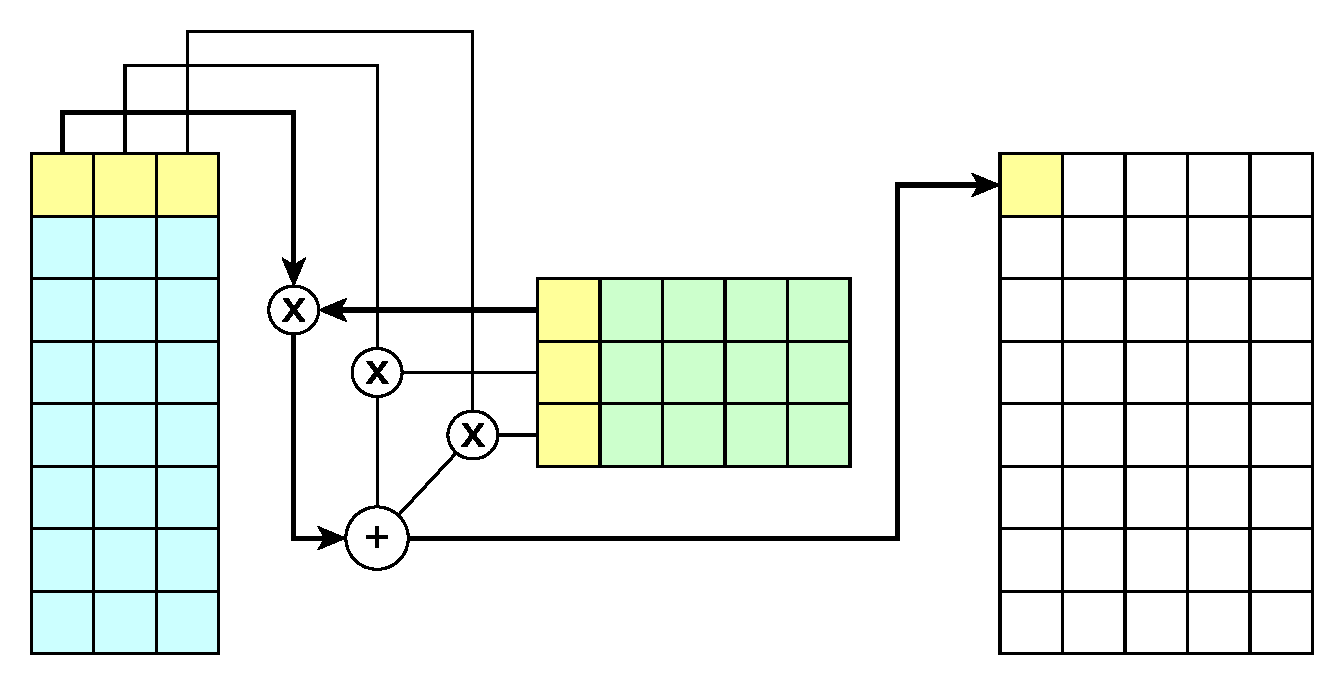
\includegraphics[width=1.0\textwidth]{pictures/iter-space-matrix.pdf}
\caption{SYCL global, local and private memory}
\label{fig:iter-space-matrix}
\end{figure}

As a first approach we can come up with simple program from (lst. \ref{lst:gemmprivate}). 

\begin{lstlisting}[caption={Naive GEMM with private memory},label={lst:gemmprivate}]
auto A = BufferA.template get_access<sycl_read>(Cgh);
auto B = BufferB.template get_access<sycl_read>(Cgh);
auto C = BufferC.template get_access<sycl_write>(Cgh);

auto Kernmul = [A, B, C, AY](cl::sycl::id<2> WorkItem) {
  const int Row = WorkItem.get(0);
  const int Col = WorkItem.get(1);

#ifdef NOPRIVATE
  for (int K = 0; K < AY; K++)
    C[Row][Col] += A[Row][K] * B[K][Col];
#else
  // this variable is workitem-private
  T Sum = 0;
  for (int K = 0; K < AY; K++)
    Sum += A[Row][K] * B[K][Col];
  C[Row][Col] = Sum;
#endif
};
Cgh.parallel_for<class mmult_naive_buf<T>>(Csz, Kernmul);
\end{lstlisting}

Here we are doing most naive matrix multiplication possible. Still results on TGLLP with and without private variable are dramatically different, see (fig. \ref{fig:plot-priv-vs-nopriv-gemm-tgllp}).

\begin{figure}
\centering
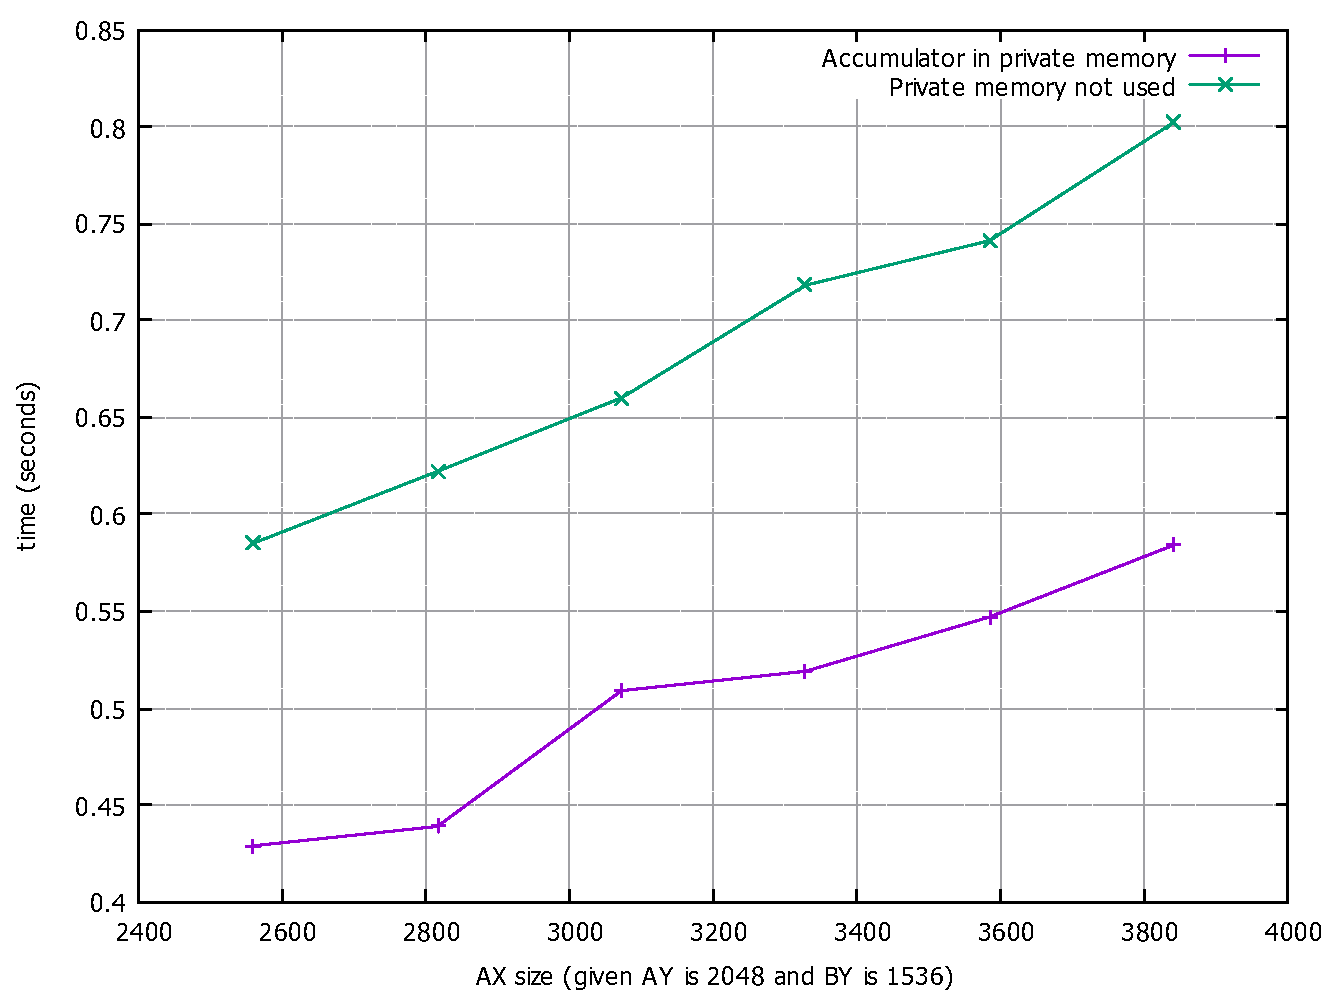
\includegraphics[width=1.0\textwidth]{pictures/plot-priv-vs-nopriv-gemm-tgllp.pdf}
\caption{TGLLP (Iris Xe) results for private memory usage for kernel from (lst. \ref{lst:gemmprivate})}
\label{fig:plot-priv-vs-nopriv-gemm-tgllp}
\end{figure}

Of course, usage of local memory for matrix multiplication improves things even more. To use it, we need local accessor, which represents something like pointer to local memory.

Main idea for listing (lst. \ref{lst:gemmlocal}) is to have a little chunk of the local memory (like 16 x 16 array). Then we tile matrix into small submatrices. Loop over tiles updates private sum for each tile. After we are done, sum becomes correct and is written to global memory.

Critical new idea here is idea of \textbf{barrier}. Barrier acts like semaphore: it stops thread and resume it after all threads will reach the barrier. In this case we are waiting for all threads in the work group.

\begin{lstlisting}[caption={GEMM with local and private memory},label={lst:gemmlocal}]
auto A = BufferA.template get_access<sycl_read>(Cgh);
auto B = BufferB.template get_access<sycl_read>(Cgh);
auto C = BufferC.template get_access<sycl_write>(Cgh);

// local memory
using LTy = cl::sycl::accessor<T, 2, sycl_read_write, sycl_local>;
LTy Asub{BlockSize, Cgh}, Bsub{BlockSize, Cgh};

auto KernMul = [=](cl::sycl::nd_item<2> It) {
  int Row = It.get_local_id(0);
  int Col = It.get_local_id(1);
  int GlobalRow = LSZ * It.get_group(0) + Row;
  int GlobalCol = LSZ * It.get_group(1) + Col;
  int NumTiles = AY / LSZ;

  T Sum = 0;
  for (int Tile = 0; Tile < NumTiles; Tile++) {
    int TiledRow = LSZ * Tile + Row;
    int TiledCol = LSZ * Tile + Col;
    Asub[Row][Col] = A[GlobalRow][TiledCol];
    Bsub[Row][Col] = B[TiledRow][GlobalCol];
    // waiting for all threads to fill Asub[Row][Col]
    It.barrier(sycl_local_fence);
    for (int K = 0; K < LSZ; K++)
      Sum += Asub[Row][K] * Bsub[K][Col];
    // waiting for all threads to use Asub[Row][Col]
    It.barrier(sycl_local_fence);
  }
  C[GlobalRow][GlobalCol] = Sum;
};
Cgh.parallel_for<class mmult_local_buf<T>>(Range, KernMul);
\end{lstlisting}

We may plot results of local memory usage on the same graph (fig. \ref{fig:plot-priv-vs-nopriv-gemm-tgllp}). We may see one more tremendous improvement.

\begin{figure}
\centering
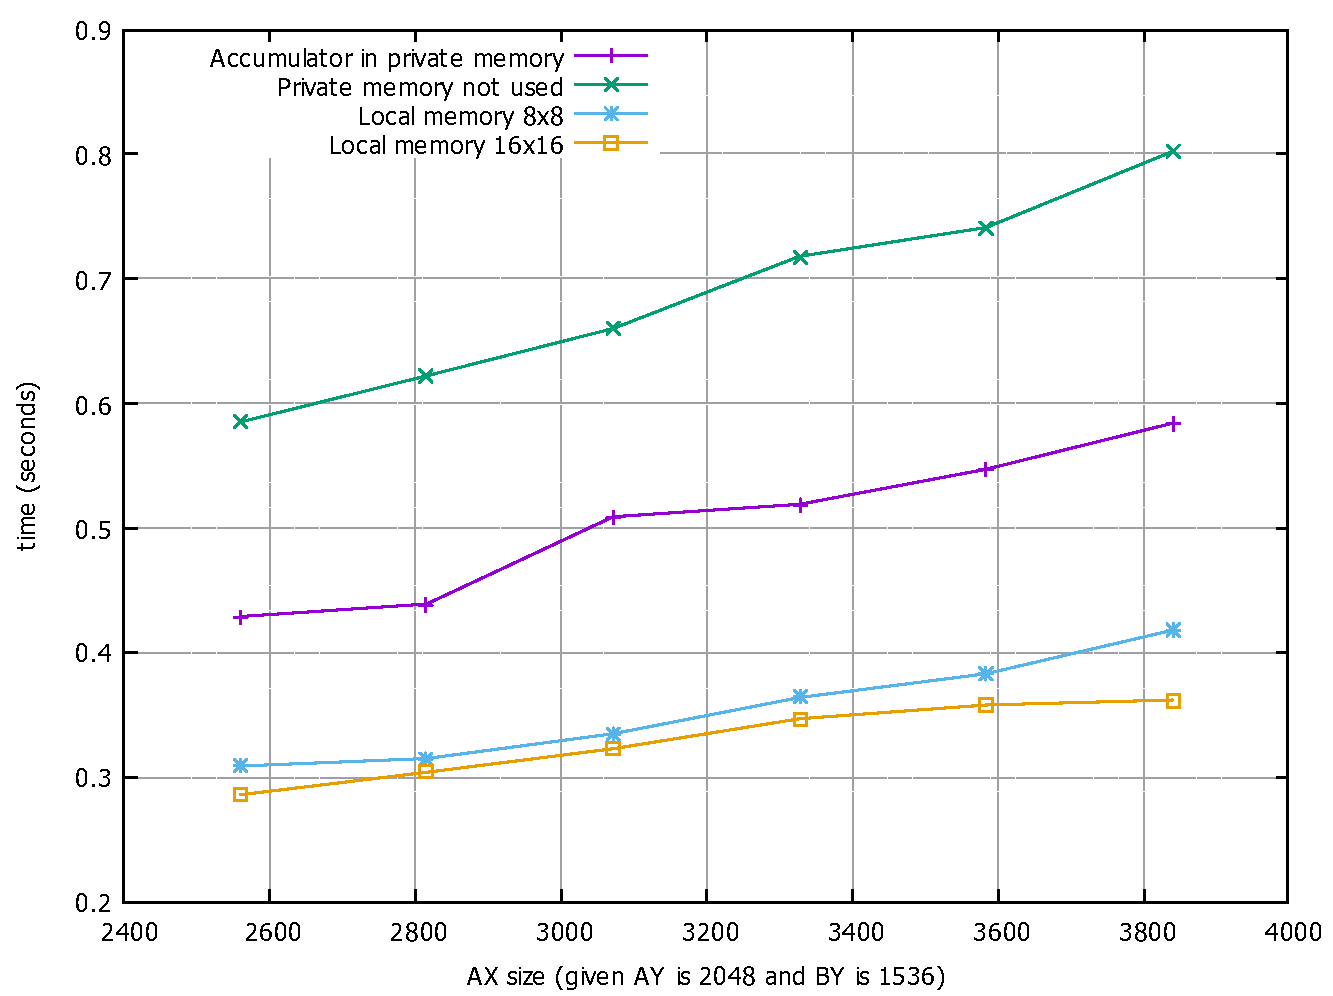
\includegraphics[width=1.0\textwidth]{pictures/plot-gemm-tgllp.pdf}
\caption{TGLLP (Iris Xe) results for local and private memory usage for GEMM}
\label{fig:plot-gemm-tgllp}
\end{figure}

Downside of explicit local memory usage is requirement for user to manually control barriers. Another interesting feature of SYCL programming is explicit hierarchical parallelism.

\begin{lstlisting}[caption={Idea of hierarchial parallelism},label={lst:gemmhiernaive}]
auto KernMul = [=](cl::sycl::group<2> Group) {
  Group.parallel_for_work_item([&](cl::sycl::h_item<2> It) {
    int GlobalRow = It.get_global_id(0);
    int GlobalCol = It.get_global_id(1);
    C[GlobalRow][GlobalCol] = 0;
  });
....
};
Cgh.parallel_for_work_group<class mmult_groups<T>>(
  NumGroups, BlockSize, KernMul);
\end{lstlisting}

Simplest idea represented on (lst. \ref{lst:gemmhiernaive}). This listing starts kernel as parallel for work group and then inside this submission runs parallel for work item. We are relying on implicit barriers between work item submissions.

We might note, that this kind of parallelism requires private memory accessor. In old way, when we used ND range, we could just have variable inside \lstinline!parallel_for! and that's all. Now things are more complicated: any private variable may live in the scope of \lstinline!parallel_for_workitem! submission only. But in order to set value of result in the end, we need some private variable, visible to any of submissions.

\begin{lstlisting}[caption={Hierarchial GEMM with private memory},label={lst:gemmhier}]
auto A = BufferA.template get_access<sycl_read>(Cgh);
auto B = BufferB.template get_access<sycl_read>(Cgh);
auto C = BufferC.template get_access<sycl_write>(Cgh);

cl::sycl::range<2> NumGroups{AX / LSZ, BY / LSZ};
cl::sycl::range<2> BlockSize{LSZ, LSZ};
const int NumTiles = AY / LSZ;

// local memory
using LTy = cl::sycl::accessor<T, 2, sycl_read_write, sycl_local>;
LTy Asub{BlockSize, Cgh}, Bsub{BlockSize, Cgh};

auto KernMul = [=](cl::sycl::group<2> Group) {
  cl::sycl::private_memory<int, 2> Sum(Group);

  Group.parallel_for_work_item(
      [&](cl::sycl::h_item<2> It) { Sum(It) = 0; });

  for (int Tile = 0; Tile < NumTiles; Tile++) {
    Group.parallel_for_work_item([&](cl::sycl::h_item<2> It) {
      int GlobalRow = It.get_global_id(0);
      int GlobalCol = It.get_global_id(1);
      int Row = It.get_local_id(0);
      int Col = It.get_local_id(1);
      int TiledRow = LSZ * Tile + Row;
      int TiledCol = LSZ * Tile + Col;

      Asub[Row][Col] = A[GlobalRow][TiledCol];
      Bsub[Row][Col] = B[TiledRow][GlobalCol];
    });

    // rely on automatic barrier

    Group.parallel_for_work_item([&](cl::sycl::h_item<2> It) {
      int Row = It.get_local_id(0);
      int Col = It.get_local_id(1);

      for (int K = 0; K < LSZ; K++)
        Sum(It) += Asub[Row][K] * Bsub[K][Col];
    });

    // rely on automatic barrier
  }

  // now assign sum to its cell
  Group.parallel_for_work_item([&](cl::sycl::h_item<2> It) {
    int GlobalRow = It.get_global_id(0);
    int GlobalCol = It.get_global_id(1);
    C[GlobalRow][GlobalCol] = Sum(It);
  });
};

Cgh.parallel_for_work_group<class mmult_groups_priv<T>>(
    NumGroups, BlockSize, KernMul);
\end{lstlisting}

To see example of private memory accessor you may want to look at (lst. \ref{lst:gemmhier}). Here we do have \lstinline!Sum! variable, declared as:

\begin{lstlisting}
cl::sycl::private_memory<int, 2> Sum(Group);
\end{lstlisting}

We can use it anywhere, accumulate things and finally use it to assign value to the output buffer in the global memory.

So logically we do have three kinds of memory (also we do have global constant one, let's forget it for now). Is it all we need to know?

Lets continue diving deeper...

\section{GPU hardware and how to think about memory}\label{sec:GPUHW}

% 1. Programming for GPU means (at least some) knowledge of architecture
% 2. Bad surprises may happen if you don't (example with too much private memory)

When you are writing code for CPU, you often need first functionality and only then (if any) performance. Say if you have obvious stall on network, or on hard drive access, any performance beyond that might not be feasible at all. So most of CPU programmers don't spend hours fighting for milliseconds, investigating generated assembler and counting cache misses (except maybe HFT and related areas).

Situation reverses when you are doing offload to GPGPU (or to any heterogeneous device). The idea of making offload means you are deliberately seeking for performance. And if you operate in SYCL only inside its logical model, you are doing things blindfold. Something may work, something not. Then you are changing your GPU and something else works, etc.

Problem is: bad surprises may happen without general understanding of what is happening under the hood.

\subsection{Stateless, stateful and local memory}\label{subsec:StatelessFull}

% 1. Idea of binding tables and stateful buffers
% 2. Stateless memory is normal memory
% 3. Local memory is a chunk of explicit cache

\subsection{Scratch, TPM and registers}\label{subsec:ScratchTPM}

% 1. Register file and GRF size estimation
% 2. Per-thread memory with hardware support (scratch)
% 3. Thread priovate memory may be no better then global buffer

\section{Full stack and how to understand your compiler}\label{sec:Compiler}

% 1. Compilers play really huge role in modern compute world
% 2. Scheme of online and offline compilation

\subsection{Stateful to stateless transformation}\label{subsec:ToStateless}

% 1. When this transformation is possible and useful
% 2. How it happens and how to block it

\subsection{Generic address space resolution}\label{subsec:GenAddr}

% 1. Motivating synthetic case
% 2. Why generic addr spaces are disaster

\subsection{Workgroups are useful}\label{subsec:Wgroups}

% 1. Implicit vectorization between threads
% 2. Stunning example in bitonic sort

\subsection{Spill means no performance}\label{subsec:Spills}

% 1. Register allocation and spills
% 2. Measures

\subsection{Memory bank conflicts}\label{subsec:Banks}

% 1. Mental model of memory bank
% 2. What is bank conflict, example

\section{Vectorization and more}\label{sec:Vectors}

% 1. Explicit SIMD and problem of inner loop vectorization
% 2. Working inside subgroup means using the whole GRF (in theory)

\subsection{Gathering accesses and Laplace equation}\label{subsec:Laplace}

% 1. Idea of gathers and scatters in hardware
% 2. Example of Laplace equation and making things better

\subsection{Explicit stateful memory}\label{subsec:Stateful}

% 1. How to force stateful memory from the host code
% 2. Why do you want it

\subsection{Samplers for compute}\label{subsec:Samplers}

% 1. Samplers and images are guests from 3D world: basic SYCL support
% 2. Can we sample any stateful buffer?

\end{document}
